\documentclass[conference]{IEEEtran}

\usepackage[T1]{fontenc}
\usepackage[utf8]{inputenc}
\usepackage{graphicx}
\usepackage{booktabs}
\usepackage{tabularx}
\usepackage{url}
\usepackage{cite}
\usepackage{balance}

\graphicspath{{figures/}}
\newcommand{\system}{Istanbul AQI Pipeline}

\title{A Distributed Streaming and Machine Learning Pipeline\\
for Real-Time Air Quality Forecasting in Istanbul}

\author{
\IEEEauthorblockN{Ahmet Can Hatipoğlu, Dicle Çoban, Funda Çelik}
\IEEEauthorblockA{
Department of Computer Engineering, Gebze Technical University\\
Big Data Analytics Course}
}

\begin{document}
\maketitle

\begin{abstract}
Urban air-quality monitoring requires both low-latency data processing and
forecasting models that can turn heterogeneous sensor observations into
actionable information. This paper presents \system, an end-to-end big-data
system for ingesting, enriching, analyzing, forecasting, and visualizing
air-quality measurements for Istanbul. The implementation combines Apache
Kafka, Apache Spark Structured Streaming, Spark MLlib, MLflow, TimescaleDB,
Grafana, and Docker Compose. A reproducible one-year synthetic benchmark
contains 263,520 hourly air-quality records from 30 stations and 8,784
city-level weather observations. The pipeline performs schema validation,
event-time weather enrichment, distributed feature engineering, historical
batch analysis, and 1-, 3-, and 6-hour AQI forecasting. On a held-out temporal
test split, the 1-hour Gradient-Boosted Trees model achieved the lowest RMSE
among the evaluated models at 86.04 AQI units, narrowly outperforming the
Random Forest and Linear Regression baselines. Error increased with forecast
horizon, reaching an RMSE of 90.88 at 6 hours. The study demonstrates a reproducible systems
prototype and identifies real-sensor validation, automated performance
benchmarking, and cloud-scale deployment as the principal remaining steps.
\end{abstract}

\begin{IEEEkeywords}
air quality, Apache Kafka, Apache Spark, structured streaming, gradient-boosted
trees, smart cities, big data analytics
\end{IEEEkeywords}

\section{Introduction}
Air pollution is an important public-health and urban-planning problem.
Fine particulate matter and other pollutants are associated with substantial
health risks, while the World Health Organization emphasizes that air-quality
management depends on reliable measurement and timely action
\cite{who_guidelines}. Istanbul presents a particularly relevant setting:
pollution varies by district, season, weather, and traffic intensity, and a
single batch-oriented view cannot adequately represent these changes.

The initial project proposal identified a gap between periodic public reporting
and the need for near-real-time situational awareness. It proposed a
Kafka--Spark pipeline that would combine Istanbul Metropolitan Municipality
(IBB), OpenAQ, and weather data; predict AQI 1, 3, and 6 hours ahead; and
present observations through a district-level dashboard. The final
implementation realizes the core local architecture and extends it with
TimescaleDB, a provisioned Grafana dashboard, MLflow experiment tracking, and a
standalone web dashboard with a Kafka-to-Server-Sent Events bridge.

This paper makes three contributions:
\begin{itemize}
    \item an end-to-end, reproducible streaming architecture that integrates
    ingestion, event-time processing, persistence, and visualization;
    \item a distributed feature-engineering and forecasting workflow with
    temporal evaluation for Linear Regression, Random Forest, and
    Gradient-Boosted Trees (GBT); and
    \item a critical evaluation of the implemented prototype, including the
    distinction between verified local functionality and proposed cloud-scale
    capabilities.
\end{itemize}

\section{Related Work}
Modern data-driven air-quality forecasting complements physically based
dispersion models by learning nonlinear relationships among pollutant history,
meteorology, time, and location. Tree ensembles are especially suitable for
heterogeneous tabular measurements because they model nonlinear interactions
without requiring the training cost and data volume of deep sequence models.
This motivated the progression from interpretable Linear Regression to Random
Forest and GBT in the present work.

The systems architecture follows established distributed-data principles.
Kafka provides a partitioned commit log for decoupled, high-throughput event
transport \cite{kafka}; Spark offers a unified engine for batch, streaming, and
machine-learning workloads \cite{spark}; and Structured Streaming provides
event-time operations and fault-tolerant incremental execution
\cite{structured_streaming}. OpenAQ demonstrates the value of harmonizing
air-quality observations behind a common data platform \cite{openaq}.

Unlike retrospective Istanbul analyses, this project focuses on integrating
stream ingestion, distributed enrichment, forecasting, experiment tracking,
and live visualization in one reproducible repository. The contribution is a
systems prototype rather than a claim of operational forecast validity.

\section{System Design}
\subsection{Architecture}
Fig.~\ref{fig:architecture} summarizes the implemented architecture. Dedicated
Python producers normalize IBB, OpenAQ, and weather payloads and publish them
to Kafka. The Docker stack provisions eight topics, including normalized
air-quality and weather topics, raw-source topics, enriched data, predictions,
and system metrics.

\begin{figure*}[t]
    \centering
    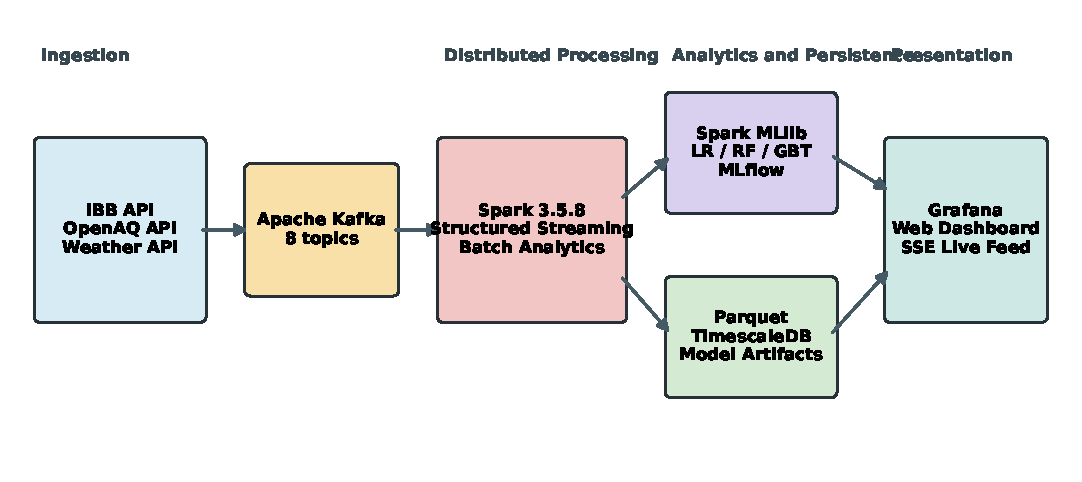
\includegraphics[width=0.96\textwidth]{architecture.pdf}
    \caption{Implemented end-to-end architecture of the \system.}
    \label{fig:architecture}
\end{figure*}

Spark Structured Streaming parses strict schemas, rejects unusable identifiers
and timestamps, and converts invalid pollutant readings to null values. Air
quality and weather streams are joined using an hourly equality bucket and a
$\pm 30$ minute event-time condition with a 35-minute watermark. This design
satisfies Spark's stream--stream join requirements while bounding state.
Enriched micro-batches are written every 30 seconds to partitioned Parquet and
TimescaleDB. Grafana is provisioned with TimescaleDB panels for current AQI,
pollutant trends, station counts, district comparisons, and AQI categories.

\subsection{Deployment and Reproducibility}
The local environment is orchestrated with Docker Compose. Table
\ref{tab:services} lists the major services. Spark jobs run with one master and
one 2-core, 2\,GB worker. MLflow records parameters and metrics. The dashboard
backend starts independent Kafka-consumer and CSV-replay workers and exposes a
pipeline-mode API; replay is explicitly enabled rather than being presented as
live data whenever Kafka is unavailable. This separation makes demonstrations
repeatable without claiming that replayed observations are real-time events.

\begin{table}[t]
\caption{Implemented Local Services}
\label{tab:services}
\centering
\begin{tabular}{lll}
\toprule
\textbf{Service} & \textbf{Role} & \textbf{Host Port}\\
\midrule
Kafka 7.6.1 & Event broker & 9092\\
Spark 3.5.8 & Batch/stream processing & 7077\\
TimescaleDB & Time-series persistence & 5432\\
Grafana 10.4.2 & Monitoring dashboard & 3000\\
MLflow 2.17.2 & Experiment tracking & 5001\\
Web dashboard & Live/SSE visualization & 8766\\
\bottomrule
\end{tabular}
\end{table}

\subsection{Interactive Dashboard and Pipeline View}
The final web dashboard adds an application-oriented presentation layer beyond
the provisioned Grafana panels. A Flask backend serves both the main dashboard
and a dedicated pipeline page and exposes station summaries, latest readings,
daily and hourly aggregates, weather records, model metrics, pipeline status,
and an SSE endpoint. The browser initializes station state through HTTP and
then updates the live feed through SSE messages forwarded from Kafka or from
CSV replay when replay is explicitly enabled through the backend API.

The main AirWatch view uses Leaflet with OpenStreetMap tiles to display
AQI-colored station markers and popups. It also presents city and station
KPIs, a sorted live feed, high-AQI alerts, Chart.js daily/pollutant/hourly
plots, station rankings, model-quality cards, and component status indicators.
The dedicated pipeline page now provides the same operational map, KPI, alert,
chart, ranking, model, and SSE-feed capabilities rather than being only a
static architecture diagram. Its CSV/Kafka toggle changes the displayed
pipeline-status sequence to distinguish batch components from streaming
components; the backend's separate pipeline-mode API controls whether replayed
or Kafka readings are forwarded. A direct AQ sink allows observations to reach
the presentation path without waiting for the weather stream join, while the
enriched stream continues to support weather-aware persistence.

\section{Data and Methods}
\subsection{Data Sources and Benchmark}
The ingestion layer supports IBB, OpenAQ, and weather APIs. Because repeatable
full-year real-source acquisition was not available during final evaluation,
the quantitative benchmark uses the repository's deterministic synthetic-data
generator with fixed random seeds. It creates 30 Istanbul stations, including
industrial and residential district profiles, for every hour of leap year
2024. Table~\ref{tab:data} describes the resulting data.

\begin{table}[t]
\caption{Evaluation Dataset}
\label{tab:data}
\centering
\begin{tabular}{lr}
\toprule
\textbf{Property} & \textbf{Value}\\
\midrule
Time range & Jan. 1--Dec. 31, 2024\\
Air-quality stations/districts & 30\\
Air-quality rows & 263,520\\
Weather rows & 8,784\\
Sampling interval & 1 hour\\
Pollutants & PM$_{10}$, PM$_{2.5}$, NO$_2$, SO$_2$, CO, O$_3$\\
Forecast targets & AQI at 1, 3, and 6 hours\\
\bottomrule
\end{tabular}
\end{table}

The generator introduces seasonal pollution, morning and evening rush-hour
peaks, district-level baselines, and random measurement variation. AQI is
computed from simplified pollutant breakpoints. Consequently, the benchmark
is useful for system and model-pipeline validation, but it must not be
interpreted as evidence of real Istanbul air quality.

\subsection{Feature Engineering}
The distributed feature pipeline first casts and validates measurements,
setting out-of-range values to null for downstream median imputation. It then
creates lag features at 1, 3, 6, 12, and 24 hours for seven pollutant/AQI
variables; 3-, 6-, and 24-hour rolling means and standard deviations; cyclic
hour, month, and weekday encodings; weekend indicators; wind-vector
components; a district index; and relative distance from central Istanbul.
Future AQI labels are generated independently within each station to avoid
cross-station leakage.

\subsection{Learning and Evaluation Protocol}
The feature table is split chronologically into 70\% training, 15\% validation,
and 15\% test periods. The primary metric is root mean squared error (RMSE);
mean absolute error (MAE) and coefficient of determination ($R^2$) provide
complementary views. Baselines are Spark MLlib Linear Regression and Random
Forest regressors for the 1-hour target. The GBT parameter search evaluates
maximum depths of 4 and 6, 20 and 50 iterations, and learning rates of 0.10 and
0.05 using three-fold cross-validation. The selected configuration---depth 4,
50 iterations, and learning rate 0.05---is reused for all horizons.

\section{Results}
\subsection{Historical Batch Analysis}
The distributed batch job produced district, hourly, weekly, monthly, and
day-of-week summaries. The synthetic benchmark displays the intended temporal
signals: mean AQI peaks at 115.71 around 08:00 and 115.56 around 18:00, while
the minimum hourly mean is 82.92 around 02:00. Monthly mean AQI is highest in
January (127.25) and lowest in July (63.96). These patterns are shown in
Fig.~\ref{fig:trends}. Because the generator explicitly encodes rush-hour and
seasonal effects, these findings validate the analytics workflow rather than
constitute empirical claims about Istanbul.

\begin{figure}[t]
    \centering
    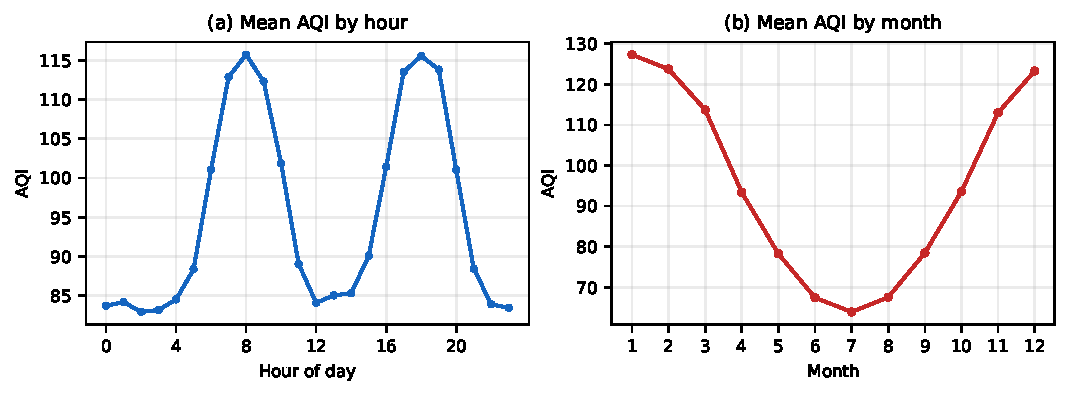
\includegraphics[width=\columnwidth]{aqi_trends.pdf}
    \caption{Temporal patterns recovered by the batch-analysis pipeline.}
    \label{fig:trends}
\end{figure}

\subsection{Forecasting Performance}
Table~\ref{tab:metrics} and Fig.~\ref{fig:models} summarize the recorded
held-out test metrics. The 1-hour GBT achieved the lowest RMSE (86.04), a
0.22\% reduction relative to Linear Regression and a 0.09\% reduction relative
to Random Forest. Linear Regression obtained the lowest MAE and classification
scores, while all models produced low $R^2$ values. Forecast quality declined
with horizon: GBT RMSE increased from 86.04 at 1 hour to 90.88 at 6 hours.
These results validate the evaluation workflow but do not meet the proposal's
predictive-performance targets.

\begin{table}[t]
\caption{Held-Out Temporal Test Performance on Synthetic Data}
\label{tab:metrics}
\centering
\begin{tabular}{lrrr}
\toprule
\textbf{Model} & \textbf{RMSE} & \textbf{MAE} & \textbf{$R^2$}\\
\midrule
Linear Regression, 1 h & 86.23 & \textbf{35.12} & 0.0594\\
Random Forest, 1 h & 86.12 & 38.54 & 0.0618\\
\textbf{GBT, 1 h} & \textbf{86.04} & 36.99 & \textbf{0.0635}\\
GBT, 3 h & 87.19 & 43.05 & 0.0399\\
GBT, 6 h & 90.88 & 46.64 & $-0.0430$\\
\bottomrule
\end{tabular}
\end{table}

\begin{figure}[t]
    \centering
    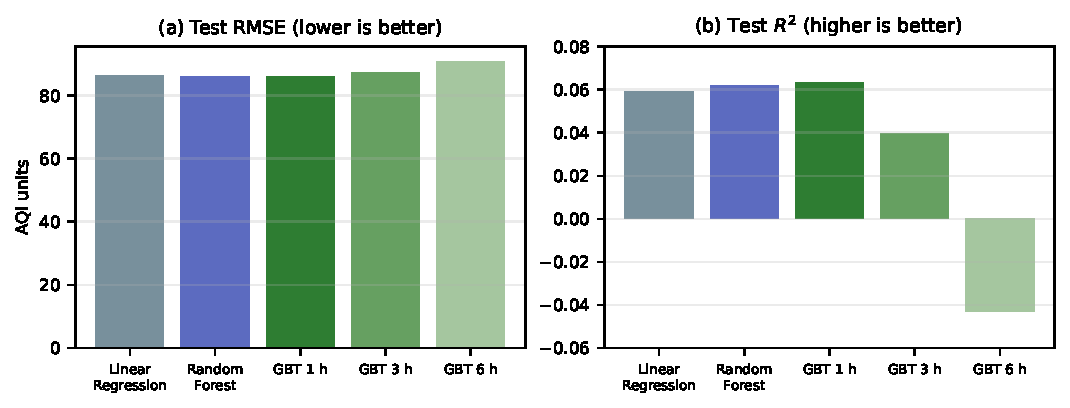
\includegraphics[width=\columnwidth]{model_results.pdf}
    \caption{Model performance by algorithm and forecast horizon.}
    \label{fig:models}
\end{figure}

\subsection{System Outcomes}
The final repository contains functioning producer contracts, Kafka topic
provisioning, Spark batch and streaming jobs, model training and inference
modules, MLflow integration, Parquet and TimescaleDB sinks, a provisioned
Grafana dashboard, and a two-page standalone web dashboard. Both web pages
provide a real Leaflet station map, live SSE feed, analytical charts, model
metrics, alerts, and pipeline-status information; the pipeline page additionally
switches between batch and streaming component views. The one-command pipeline
orchestrates historical analysis, baseline training, GBT training, and
evaluation. These outcomes satisfy the central objective of demonstrating an
integrated big-data workflow.

The proposal also defined latency below 120 seconds, throughput above 500
records/s, executor-scaling experiments, AWS deployment, and a live
district-level prediction map as success criteria. Configuration and
deployment guides exist, and the streaming trigger is 30 seconds, but no
controlled latency, throughput, scaling, or AWS benchmark artifact is present.
Therefore, these targets are not reported as achieved.

\section{Discussion}
The results show that the implementation can recover designed temporal
patterns and train distributed forecasting models on the deterministic
benchmark. GBT provides the best 1-hour RMSE, although its improvement over the
baselines is small and the low $R^2$ values show that predictive performance
remains insufficient. The gradual degradation from 1 to 6 hours is consistent
with increasing forecast uncertainty.

Several limitations constrain interpretation. First, synthetic data embed
smooth seasonal and rush-hour functions and therefore make the forecast task
more regular than real sensor data. Second, the current weather series is
city-wide rather than station-specific. Third, no controlled comparison of
partition counts, executors, latency, throughput, or fault recovery has been
archived. Fourth, the automated test files currently establish only placeholder
contracts, leaving important integration behavior insufficiently protected.
Fifth, the pipeline page's visible CSV/Kafka toggle changes its status
presentation but does not call the backend pipeline-mode API; replay activation
therefore requires a separate API request. Finally, future runs should emit
immutable, timestamped evaluation manifests and associated MLflow run
identifiers.

These limitations suggest a clear next evaluation phase: acquire a continuous
real-data window from IBB and OpenAQ, archive raw payloads, use rolling-origin
evaluation, compare against persistence and seasonal-naive baselines, record
MLflow run identifiers with every table, and benchmark the streaming path
under controlled Kafka load at multiple Spark executor counts.

\section{Conclusion}
This paper presented an end-to-end big-data prototype for real-time air-quality
monitoring and forecasting in Istanbul. The implemented system unifies Kafka
ingestion, Spark Structured Streaming, distributed batch analytics, Spark
MLlib forecasting, MLflow tracking, TimescaleDB persistence, and Grafana/web
visualization. On a reproducible one-year synthetic benchmark, the 1-hour GBT
model achieved the lowest RMSE at 86.04, while performance degraded at longer
horizons and the predictive targets were not met. The main result is a functioning and
reproducible systems foundation. Establishing operational value now requires
real-sensor validation, stronger automated tests, immutable experiment
artifacts, and measured cloud-scale performance.

\section*{Acknowledgment}
The authors thank Dr.\ Salih Sarp for his guidance in the Big Data Analytics
course and acknowledge IBB and OpenAQ for providing open environmental-data
interfaces that motivated the system design.

\balance
\begin{thebibliography}{00}
\bibitem{who_guidelines}
World Health Organization, \emph{WHO Global Air Quality Guidelines:
Particulate Matter (PM$_{2.5}$ and PM$_{10}$), Ozone, Nitrogen Dioxide,
Sulfur Dioxide and Carbon Monoxide}. Geneva, Switzerland: WHO, 2021.

\bibitem{kafka}
J. Kreps, N. Narkhede, and J. Rao, ``Kafka: A distributed messaging system
for log processing,'' in \emph{Proc. NetDB}, Athens, Greece, 2011, pp. 1--7.

\bibitem{spark}
M. Zaharia \emph{et al.}, ``Apache Spark: A unified engine for big data
processing,'' \emph{Commun. ACM}, vol. 59, no. 11, pp. 56--65, Nov. 2016.

\bibitem{structured_streaming}
M. Armbrust \emph{et al.}, ``Structured Streaming: A declarative API for
real-time applications in Apache Spark,'' in \emph{Proc. ACM SIGMOD},
Houston, TX, USA, 2018, pp. 601--613.

\bibitem{openaq}
OpenAQ, ``OpenAQ platform and API documentation,'' 2026. [Online].
Available: \url{https://docs.openaq.org/}

\bibitem{mllib}
X. Meng \emph{et al.}, ``MLlib: Machine learning in Apache Spark,''
\emph{J. Mach. Learn. Res.}, vol. 17, no. 34, pp. 1--7, 2016.

\bibitem{mlflow}
M. Zaharia \emph{et al.}, ``Accelerating the machine learning lifecycle with
MLflow,'' \emph{IEEE Data Eng. Bull.}, vol. 41, no. 4, pp. 39--45, 2018.
\end{thebibliography}

\end{document}
